\chapter{Detector commissioning}
\label{sec:commissioning}

By the end of $2019$, the commissioning of the SuperNEMO demonstrator has begun and first calorimeter data were taken.\\
To clarify, we give some common terms used in the detector assembly.
The calorimeter of SuperNEMO is segmented in $712$ optical modules (OM), each composed by a coupling between a photomultiplier tube (PMT) and a polystyrene scintillator (see sec.~\ref{sec:calorimeter} for more details).
The divider of a PMT is connected to $2$ cables, one providing the high voltage (HV), the other one, called signal cable, is a coaxial cable collecting and transporting the charge provided by the PMT.\\
By the summer $2020$, the SuperNEMO demonstrator will be encapsulated in an anti radon tent (\textcolor{red}{abbrev?}).
The so called \emph{patch panel} (PP) will insure passage of cables from inside, to outside the anti radon tent, therefore doubling the amount of cables needed for the calorimeter.
We commonly talk about \emph{internal} cables (from detector to patch panel) and \emph{external} cables (from patch panel to electronics).
Consequently, regarding only the calorimeter part, 2848 cables were cut, assembled, connector-mounted, transported and installed at Modane.
Then checking cables condition is mandatory to control and eventually fix the cables.

\section{Reflectometry tests}
\label{sec:reflecto}

\subsection{Principle and goal}

Taking into account the final demonstrator design, each coaxial cable length were determined, then cables were cut and labelled in LAL, Orsay.
To check if the cables were cut at right length and if no inversions were made at Modane when connecting them, we want to verify each cable length after installation.
To do so, a channel at electronic boards send a pulse, called \emph{primary} pulse, in the connected cable.
The signal will travel from electronics to the PMT through this coaxial cable.
As the PMT is not alimented (the HV is turned off during this data taking), the impedance at the PMT is infinite, and the signal reflects at the PMT divider.
Then the signal travels back from the PMT to the channel at electronic boards, were it will be recorded by the acquisition.
We called this recorded back pulse \emph{secondary} pulse.
Analysing the shape and arrival time of those secondary pulses will allow us to check coaxial cable conditions and control their lengths.

\subsection{Data taking at LSM}
\textcolor{red}{Explain the pulse sending principle with Jihane's documentation}

\subsection{Pulse timing: controlling cable lengths}
\label{subsec:timing}

After all cables were transported to Modane, to determine precisely each coaxial cable length is important for three reasons:
\begin{itemize}
\item to control if no inversions were made during calorimeter cabling: all external coaxial cable is $7$ meters-long (the distance between electronics and patch panel being the same for all channels), but internal cables length have been adapted to fit the distance from the patch panel to each optical module;
\item to check if cables were cut at right length;
\item to estimate the delay of signal due to cable lengths: the velocity of electrons in cables has a regular value that delays the signal comming from the PMT. This time delay depends on the cable length and has to be characterised for each electronic channel.
\end{itemize}
In order to do this, we determine the difference between primary pulse and secondary pulse times.
Knowing the velocity of electrons in coaxial cables, we can deduce the corresponding cable length.
This measure is repeated for each PMT, allowing us to characterise all coaxial cables.\\
The propagation velocity of electrons in coaxial cables, $v_{p}$, is a parameter given as a fraction of the light speed in vaccuum, $c$, as
\begin{equation*}
  v_{p}=\frac{1}{\sqrt{\epsilon}}\,\text{,}
\end{equation*}
with $\epsilon$ the dielectric constant of the material.
For the coaxial cables chosen for the demonstrator, this velocity is $0.69c$.

We define the time of a pulse with a Constant Fraction Discriminator (CFD) parameterised by the fraction $f$, as represented in fig.~\ref{fig:CFD}.
\textcolor{red}{expliquer CFD dans texte}
We studied the influence of this fraction on the time measurement precision (see Sec.~\ref{subsec:CFD}).
In the following, we use $\text{f} = 40\%$.
The cable length $\mathcal{L}$ is therefore defined as $\mathcal{L}= 0.5\,\mathcal{T}\,v_{p}$, with $\mathcal{T}$ the round trip time from electronics to PMT divider, defined as
\begin{equation}
\mathcal{T} = \braket{\text{t}_{\text{secondary pulse}}-\text{t}_{\text{primary pulse}}}_{\text{p}} \, \text{,}
\end{equation}
$\braket{}_{\text{p}}$ being the average over all pulses sent in one cable, and $t_{i}$ the time of pulse $i$.
We repeat this operation for all electronic channels so all cables are controlled and characterised.
A study was also performed to experimentally confirm electron celerity in the used coaxial cables (see Sec.~\ref{subsec:velocity}).

The principal aim of this study is to control if cables were correctly cut, following the initial design.
Therefore, we define $l^{d}_{j}$ as the initial designed length for a given cable $j$, and $l^{m}_{j}$ the cable length measured by reflectometry for a cable $j$.
Hense the length difference $\Delta L_{j}$ for a cable $j$ is defined as:
\begin{equation}
  \Delta L_{j} = l^{m}_{j}-l^{d}_{j}\, .
\end{equation}
On Fig.~\ref{fig:LengthDiff} is displayed the distribution $\Delta L$ for all the measured coaxial cables.
\begin{figure}
  \centering
  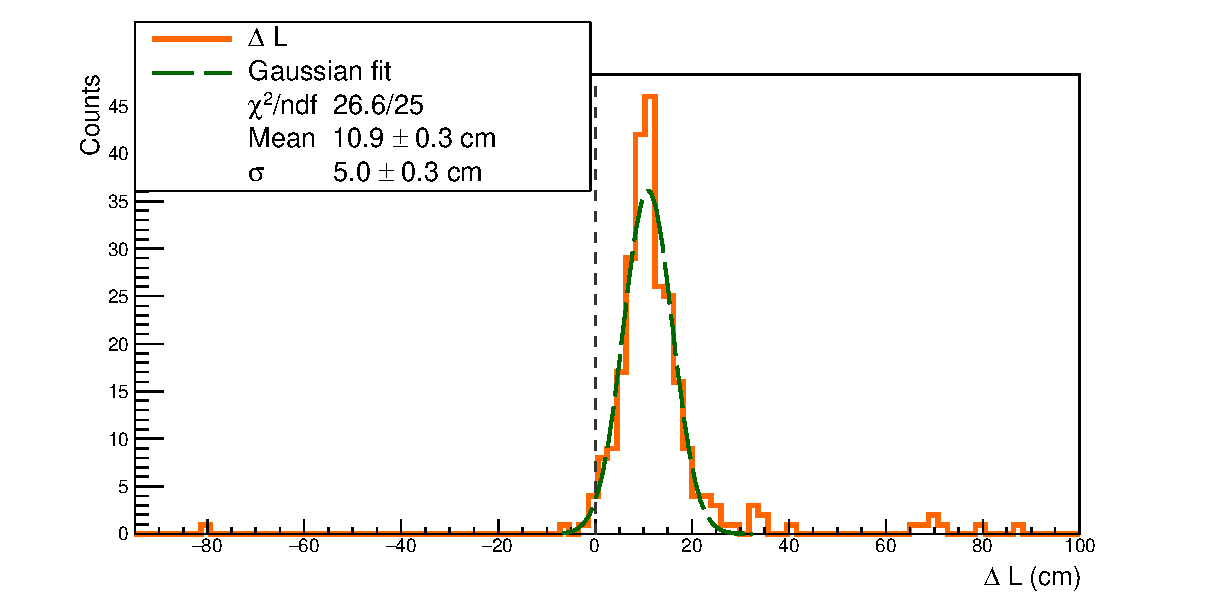
\includegraphics[width=15cm]{commissioning/fig_commissioning/length_diff.eps}
  \label{fig:LengthDiff}
  \caption{The distribution of difference between measured length (by reflectometry) and expected length is displayed in orange plain line.
  The gaussian fit (red dashed line) has a mean of $10.9 \pm 4.9$ cm.}
\end{figure}
In hypothetical perfect conditions, all the cables $j$ should have the designed length, in other words, $l^{d}_{j} = l^{m}_{j}$.
Consequently the $\Delta L$ distribution should be a Dirac peak centered at $0$, as materialised by the black dashed line.
However, in real conditions, the measured length can be different from the designed one, leading to a gaussian distribution plotted in orange plain line.
A gaussian fit (green dashed line) performed on this $\Delta L$ distribution point out a $\sigma$ value of $4.9$ cm, revealing the precision of the cutting device.
The mean value of the gaussian fit is also interesting, with $10.9$ cm, meaning that cables are longer than expected in average.
This may reveal a bias coming from the device used to cut the cables.
On Fig.~\ref{fig:CutBias} is plotted the length difference $\Delta L$ with the initial designed length $l^{d}$ (greened blue).
A linear fit parameterised by $y = \alpha x + \beta$, is displayed in orange plain line.
\begin{figure}
  \centering
  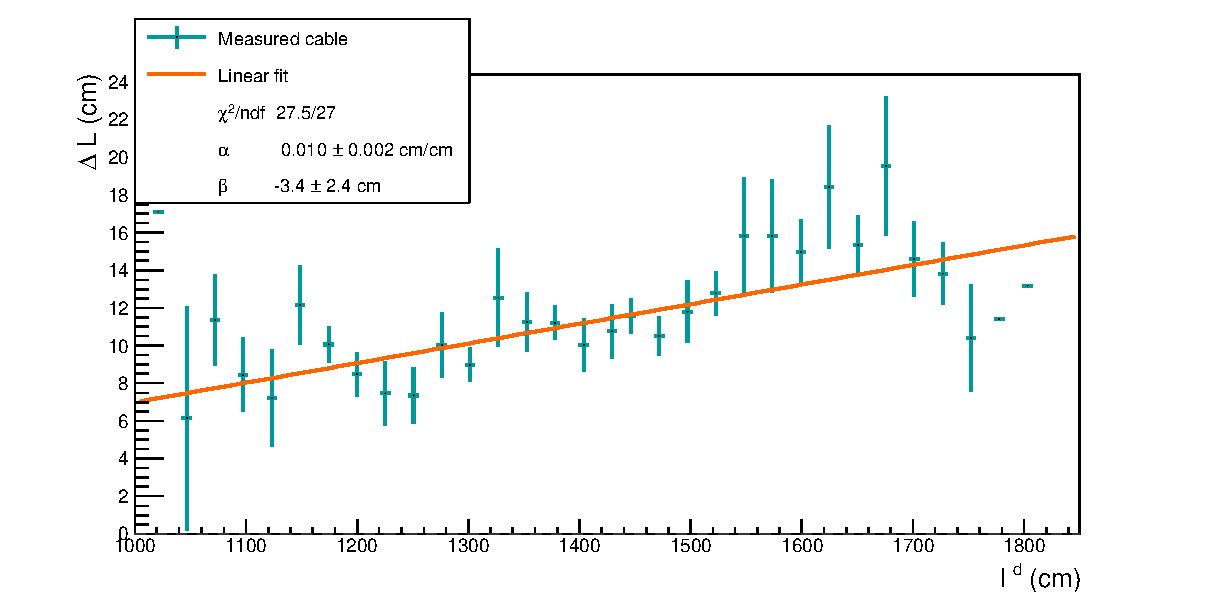
\includegraphics[width=15cm]{commissioning/fig_commissioning/cut_biais.eps}
  \label{fig:CutBias}
  \caption{}
\end{figure}
The $y$-intercept of this linear fit, reprensented by the parameter $\beta$, shows that the cutting devide systematically take away $-4.1$ cm of each cable.
Besides, the slope of the linear fit, $\alpha$, reveals a slight bias of the cutting device, adding $1$ cm every meter of cable.
This bias would have been a problem with a negative slope, in other words, if measured cable lengths were systematically smaller than the designed ones, leading to eventual connection issues to PMT.
However, we can notice that some cables have been cut shorter, one of them being $80$ centimenters shorter than expected.
Hopefully, this cable were checked at LSM, showing it was succefully connected to PMT despite this deficit.

This study allowed us to control and record the lengths of all coaxial cables installed on the SuperNEMO demonstrator at LSM.
In addition, reflectometry also aimed at checking the cable condition by performing waveform shape anaysis on secondary pulses.

Rq: controlling the length do not include that the cable is connected (reflection can occur at the end of the cable).


\subsection{Correction on event times}
\label{subsec:time_correction}

The main goal of this study was to check the lengths of coaxial cables.
We can also use the results to correct the time of recorded events.
Given that what we later define as an \emph{event} is firstly an electric signal, we should take into account the time for the signal to travel through cables.
This become possible with the reflectometry study we performed.
Knowing real lengths of cables and using the celerity of the signal, we deduce the time needed for the signal to travel from one given PMT divider to the electronics.
Then we can correct event times.


\subsection{Checking the pulse amplitude attenuation}
When the signal travels in a cable, its amplitude is attenuated.
Then, another test for controlling the cable condition is to check if this attenuation matches the expectations (i.e. the value given by constructor).
We define the amplitude of a pulse as the maximum of this pulse, compared to the baseline.
The attenuation $\mathcal{A}$ of a given cable is then defined as $\mathcal{A}=\braket{\text{A}_{ \text{secondary pulse}}-\text{A}_{ \text{primary pulse}}}_{\text{p}}$, $\text{A}_{\text{i}}$ the amplitude of the pulse i.
A map summarising the attenuation for each cable is presented.

\subsection{Checking the constructor signal velocity in cables}
\label{subsec:velocity}
As we want to check the celerity of signal given by Axon, we used $3$ cables of different lengths (see Fig.~\ref{fig:cable_lengths}).
Knowing the length of a cable, we determine the time needed for the signal to make a round trip in the cable, and conclude about the celerity of signal in each cable.
We found that the mean celerity on the $3$ cables is $0.7$ c, a bit greater than the celerity given by Axon of $0.69$ c.


\subsection{Studying influence of CFD on the signal timing study}
\label{subsec:CFD}

\subsection{Pulse shape analysis}
\label{subsec:pulse_shape}


\subsection{Results}



\section{Calibrating the electronics}
\label{sec:TimeSynchroFEB}

\subsection{Principle}
\subsection{Measuring the time offset of front end boards}
\subsection{Results}

\begin{figure}
  \centering
  \includegraphics[width=10cm]{commissioning/fig_commissioning/CFD_example.pdf}
  \label{fig:CFD}
  \caption{In black is an example of a waveform with primary pulse (left) and secondary pulse (right).
    A representation of time CFD is given for the secondary pulse.
    Its maximal amplitude (red dotted line) and its fraction for $\text{f}=40\%$ (green dotted line) are displayed.
    The time $\text{T}_{\text{pulse}}$ (orange dotted line) reprensents the time of the secondary pulse calculated with a CFD at $\text{f}=40\%$.}
\end{figure}

\begin{figure}
  \centering
  \includegraphics[width=10cm]{commissioning/fig_commissioning/length_tests.pdf}
  \label{fig:cable_lengths}
  \caption{Primary and secondary pulses for a $698 \pm 1$ cm cable (green), a $1043 \pm 1$ cm cable (red) and a $2025 \pm 1$ cm cable (grey).}
\end{figure}
